\documentclass[12pt]{article}
\usepackage{tempora}
\usepackage[utf8]{inputenc}
\usepackage[T2A]{fontenc}
\usepackage{cmap}
\usepackage{mathtext}
\usepackage{array}
\usepackage{booktabs}
\usepackage{multirow}
\usepackage[russian,english]{babel}

\usepackage{amsmath,amsfonts,amssymb,amsthm,mathtools} % AMS
\usepackage{icomma}

\usepackage[left=10mm, top=20mm, right=18mm, bottom=15mm, footskip=10mm]{geometry}
\usepackage{indentfirst}
\usepackage{euscript}	 % Шрифт Евклид
\usepackage{mathrsfs} % Красивый матшрифт

\usepackage[italicdiff]{physics}
\usepackage{graphicx}
\graphicspath{{images/}}
\DeclareGraphicsExtensions{.pdf,.png,.jpg}
\usepackage{wrapfig}
\usepackage{subcaption}
\usepackage{caption}
\usepackage{hyperref}
\usepackage[rgb]{xcolor}



\hypersetup{				% Гиперссылки
    colorlinks=true,       	% false: ссылки в рамках
	urlcolor=blue          % на URL
}
\captionsetup[figure]{name=Рисунок}
\captionsetup[table]{name=Таблица}


% Определяем команду для строки оглавления с отточками
\newcommand{\tocline}[2]{%
  \noindent\makebox[0pt][l]{#1}\hfill
  \leaders\hbox to 1.5mm{\hss.\hss}\hfill
  \makebox[0pt][r]{#2}\par
}

% Альтернативный стиль (более надёжный, работает всегда):
\newcommand{\tocentry}[2]{%
  \noindent
  \parbox[t]{0.8\textwidth}{\raggedright #1}%
  \parbox[t]{0.15\textwidth}{\raggedleft #2}%
  \par
  \vspace{-1.2\baselineskip}
  \noindent\leaders\hbox to 1.5mm{\hss.\hss}\hfill\mbox{}%
  \par
  \vspace{0.8\baselineskip}
}

% Но самый простой и надёжный способ — через \dotfill:
\newcommand{\tocitem}[2]{%
  \noindent #1 \dotfill\ #2\par
}


\begin{document}

\thispagestyle{empty}

\begin{center}

% Верхняя часть титульного листа
\large
Министерство науки и высшего образования Российской Федерации \\
\large
ФЕДЕРАЛЬНОЕ ГОСУДАРСТВЕННОЕ АВТОНОМНОЕ \\
ОБРАЗОВАТЕЛЬНОЕ УЧРЕЖДЕНИЕ ВЫСШЕГО ОБРАЗОВАНИЯ \\
\large
«МОСКОВСКИЙ ФИЗИКО-ТЕХНИЧЕСКИЙ ИНСТИТУТ \\
(НАЦИОНАЛЬНЫЙ ИССЛЕДОВАТЕЛЬСКИЙ УНИВЕРСИТЕТ)» \\
(МФТИ, Физтех)

\vspace{3cm}

% Основная информация
\large
КАФЕДРА ЭЛЕКТРОНИКИ

\vspace{0.7cm}

\Large
ОТЧЕТ \\
ПО ЛАБОРАТОРНОЙ РАБОТЕ

\vspace{0.7cm}

\Large
\textbf{Волоконный лазер}

\vfill

\vspace{1.5cm}
% Блок с подписями

\large

\noindent
Работу выполнили \hfill \underline{\hspace{6cm}} Д.А.Воронин Б04-407 \\
\hfill {\small (подпись, дата)}\par % <-- ИСПРАВЛЕНО ЗДЕСЬ


\noindent
\hfill \underline{\hspace{6cm}} Т.А.Ганицев Б04-407 \\
\hfill {\small (подпись, дата)}\par % <-- И ЗДЕСЬ

\noindent
\hfill \underline{\hspace{6cm}} Н.Л.Кеткин Б04-407 \\
\hfill {\small (подпись, дата)}\par % <-- И ЗДЕСЬ

\noindent
\hfill \underline{\hspace{6cm}} С.А.Стряпко Б04-407 \\
\hfill {\small (подпись, дата)}\par % <-- И ЗДЕСЬ

\noindent
\hfill \underline{\hspace{6cm}} Девочка из Б04-405? \\
\hfill {\small (подпись, дата)}\par % <-- И ЗДЕСЬ

\vspace{3cm}

\noindent
Работу принял, оценка \hfill \underline{\hspace{6cm}} \\
\hfill {\small (подпись, дата, оценка)} % <-- И ЗДЕСЬ

\vfill

% Нижняя часть
Долгопрудный 2026

\end{center}

\newpage

\thispagestyle{empty} % Убираем номер страницы с листа оглавления
\renewcommand{\contentsname}{ОГЛАВЛЕНИЕ} % Меняем заголовок (по желанию)
\tableofcontents
\newpage
\section{Цель работы}

    \begin{enumerate}
        \item Основываясь на скоростных балансных уравнениях, рассчитать основные параметры генерации лазера. 
        \item Изучить генерацию в волоконном лазере в режиме свободной генерации и физические основы появления релаксационных колебаний.
        \item Измерить энергетические параметры выходного излучения.
        \item Изучить методы создания инверсии, управления режимами генерации и формирования модовой структуры излучения в лазере.
        \item Определить влияние параметров генерации на частоту и затухание релаксационных колебаний.
    \end{enumerate}


\section{Теоретические сведения}

\subsection{Об волоконном лазере}

Впервые волоконный лазер был создан в 1963 году. Волоконный свотовод длинной 1 м содержал ионы неодима и служил в качестве активной усиливающей среды. Для накачки использовалась дуговая лампа. Но существенное развитие этого типа лазеров

произошло после создания волоконных световодов с малыми потерями и полупроводниковых лазеров, способных обеспечить необходимую мощность накачки.

\par

В качестве активных ионов могут быть использованы только те, у которых энергетический зазор между уровнями с оптическими переходами превышает величину 400 - 1100 $\text{см}^{-1}$ иначе безизлучательная релаксация привеедет к ухудшению люминисценции.

Наиболее часто берут неодим, гольмий, эрбий, тулий, иттербий.

\par

Структура энергетических уровней иттербия, используемых в лазере, состоит из двух уровней~--- основного ${}^2\mathrm{F}_{7/2}$ и ${}^2\mathrm{F}_{5/2}$~--- метастабильного, которые расщеплены вследствие эффекта Штарка, что и приводит к сложной форме полосы поглощения и люминесценции.\par

Поглощение имеет два максимума с длинами волн 915 и 976~нм, что и обуславливает выбор источника полупроводниковой накачки. Люминесценция имеет максимумы в областях 978--982~нм и 1030--1040~нм. Время жизни метастабильного уровня для ионов иттербия в фосфатном волокне составляет 1,4~мс.

\par

Преимущества волоконных активных сред по сравнению с объемными активными лазерными средами:
\begin{itemize}
    \item низкие оптические потери;
    \item большая длина взаимодействия и малый размер световедущей сердцевины, что обеспечивает эффективную накачку полупроводниковым лазером;
    \item большое отношение площади поверхности волокна к объему, что улучшает теплоотвод;
    \item высокое качество поперечной структуры пучка;
    \item использование внутриволоконных брегговских решеток в качестве распределенных зеркал обеспечивает компактность и стабильность лазера.
\end{itemize}

\newpage

\subsection{Инверсия активной среды}

Излучение лазера рождается на переходах между определенными энергетическими уровнями активных центров; их называют $\textbf{рабочими уровнями}$. Отнесенные к единице объема активной среды заселенности рабочих уровней будем обозначать через $n_1$ (нижний рабочий уровень) и $n_2$ (верхний рабочий уровень). Разность
\[
H = n_2 - (g_2/g_1)n_1 \tag{1}
\]

называют 
\emph{плотностью инверсной заселенности рабочих уровней}. 


Здесь $g_1$ и $g_2$ -- кратности вырождения соответствующих уровней; для простоты будем, как правило, полагать, что $g_1 = g_2$.

Если выполняется условие
\[
N(t,x,y,z) > 0\,, \tag{2}
\]
то говорят, что имеет место $\textbf{инверсия активной среды}$.
\par
Коэффициент усиления $\chi_1$ пространственно-однородной среды описывается выражением
\[
\chi_1 = \sigma N\,,\tag{3}
\]

где $\sigma$~--- сечение вынужденных переходов между рабочими уровнями.

\par

Для создания и поддержания инверсии применяют тот или иной способ возбуждения активной среды. Активная среда лазера представляет собой некий термостат (сердцевина волокна из стекла), в котором имеются активные центры~--- квантовые системы, способные в результате возбуждения переходить в состояние с отрицательной температурой, отвечающей инверсной заселенности уровней.

В твердотельных волоконных лазерах активными центрами чаще всего служат ионы с незаполненными внутренними оболочками.

\par

\textbf{Плотность светового потока}:

\[
dS_\omega = [\chi_1(z) - \chi_2] S_\omega(z) dz\,.\tag{4}
\]

где
\begin{itemize}
    \item $\chi_1$ - коэффициент оптического усиления
    \item $\chi_2$ - коэффициент поглощения на неактивных центрах и рассеяния
\end{itemize}

Таким образом, при достаточно больших $z$ при условии $\chi_1(z) > \chi_2$, когда среда является усиливающей, возможна генерация оптического излучения.

\par

Для осуществления режима генерации нужно создать \textbf{положительную обратную связь}.


\subsection{Получение инверсной заселенности}

\textbf{Когерентная оптическая накачка} предполагает возбуждение активных центров при поглощении активной средой излучения от специального источника света.

Излучение накачки со специально подобранным спектром частот позволяет возбуждать отдельную группу уровней или отдельный уровень.

При когерентной накачке лазер можеть быть как \textbf{усилитель когерентного излучения} так и \textbf{преобразователем оптических частот}.

\par

Для ввода излучения накачки используются:

\begin{itemize}
    \item торцевой метод
    \item набор V - образных канавок
    \item два световода: активный и тот в который вводится излучение накачки
\end{itemize}

\newpage

\subsection{Режим свободной генерации}

\textbf{Режим свободной генерации} означает отсутствие какого - либо специального упрваления генерацией и воздействия на нее из вне. Она может быть и в случае импульсной и в случае непрерывной накачки.

\par

Свободное излучение волоконного лазера представляет собой, как правило, последовательность относительно коротких импульсов или пичков. Длительность отдельного пичка равна $10^{-7}$--$10^{-6}$~с (0,1--100~мкс); мощность достигает значений $10^1$--$10^2$~Вт. Временной интервал между пичками составляет примерно 1--10~мс.

\begin{figure}[h]
    \centering
    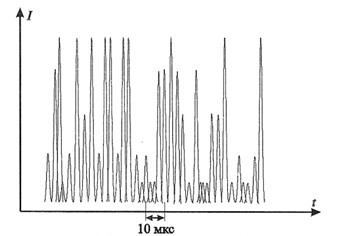
\includegraphics[width=10cm]{p1.png}
    \caption{Осцилограмма излучения лазера в режиме свободной генерации}
    \label{img_energy_levels}
\end{figure}

\subsection{Система уравнений, описывающих динамику генерации лазера}

\begin{figure}[h]
    \centering
    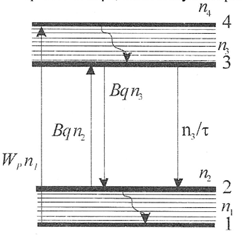
\includegraphics[width=8cm]{p2.png}
    \caption{Энергетическая схема квази - четырехуровнего лазера}
    \label{img_energy_levels}
\end{figure}

\newpage

Считая, что переходы между уровнями 4 и 3 и уровнями 2 и 1 являются быстрыми, можно положить $n_4 \approx n_2 \approx 0$. В этом случае скоростные уравнения можно записать следующим образом:

\[
\begin{cases}\tag{5}
\dfrac{dn_3}{dt} = W_p n_1 - B q n_3 - \dfrac{n_3}{\tau}, \\[10pt]
\dfrac{dq}{dt} = V_a B q n_3 - \dfrac{q}{\tau_c}, \\[10pt]
n_1 + n_3 = N_t,
\end{cases}
\]

где
\begin{itemize}
    \item $N_t$~--- полное число активных атомов в единице объема,
    \item $n_1$~--- населенность основного состояния,
    \item $n_3$~--- населенность рабочего уровня,
    \item $q$~--- полное число фотонов в резонаторе,
    \item $W_p$~--- скорость накачки,
    \item $\lambda = 1{,}064$~мкм~--- длина волны генерации,
    \item $\tau = 1400$~мкс~--- время жизни рабочего уровня,
    \item $\tau_c = L'/\gamma c$~--- время жизни фотонов в резонаторе,
    \item $\gamma$~--- потери в резонаторе за проход в одном направлении,
    \item $V_a = \pi \omega_0^2 l / 4$~--- объем моды в активной среде,
    \item $B$~--- скорость индуцированных переходов на один фотон в моде,
    \item $\omega_0$~--- размер перетяжки моды в резонаторе,
    \item $L$~--- длина резонатора,
    \item $l$~--- длина активной среды,
    \item $L' = L + (n_0 - 1)l$~--- оптическая длина резонатора,
    \item $n_0$~--- показатель преломления активной среды,
    \item $c = 2{,}99792458 \times 10^{10}$~см/с~--- скорость света,
    \item $N = 8 \times 10^{19}$~ионов/см$^3$~--- плотность ионов Yb${}^{3+}$.
\end{itemize}

Выражения для введенных величин $B$ и $\tau_c$ через известные параметры лазера:
\[
B = \frac{\sigma c}{V_a L'} = \frac{\sigma c}{V}, \qquad \tau_c = \frac{L'}{c\gamma},\tag{6}
\]
где $V = \pi\omega_0^2 L'/4$~--- объем моды в резонаторе.

\newpage

Вводя инверсную населенность уровней 3 и 2 по формуле $N = n_3 - n_2 \approx n_3$, систему уравнений (5) можно переписать в виде
\[
\begin{cases}\tag{7}
\dfrac{dN}{dt} = W_p (N_t - N) - B q N - \dfrac{N}{\tau}, \\[10pt]
\dfrac{dq}{dt} = \left( B V_a N - \dfrac{1}{\tau_c} \right) q,
\end{cases}
\]

\textbf{Пороговое условие генерации лазера}

\par

Чтобы $\dfrac{dq}{dt}$ было положительным нужно $(V_a B N - 1/\tau_c) > 0$. В этом случае генерация возникнет, если инверсия превысит \textbf{критическое значение $N_c$}, определяемое выражением
\[
N_c = \frac{1}{V_a B \tau_c} = \frac{\gamma}{\sigma l},\tag{8}
\]

где
\begin{itemize}
    \item $\sigma$~--- сечение перехода генерации (эффективное сечение перехода генерации для ионов Yb${}^{3+}$: $\sigma = 2{,}5 \times 10^{-20}$~см${}^2$),
    \item $\gamma$~--- суммарные потери в резонаторе за проход в одном направлении, определяемые ниже.
\end{itemize}

В итоге \textbf{критическая скорость накачки} возникае при равенстве полной скорости накачки $W_{cp} (N_t - N_c)$ и скорости $N_c/\tau$ спонтанных переходов:
\[
W_{cp} = \frac{N_c}{(N_t - N_c)\tau}.\tag{9}
\]

\textbf{Пороговая скорость накачки уровней}:

\[
W_{cp} = \frac{1}{\tau(\tau_c V_a B N_t - 1)}.\tag{10}
\]

Если $W_{p}$ > $W_{cp}$ то q достигнет постоянного значения $q_{0}$ и соответствующее $N_{0}$ 

\[\tag{11}
\begin{aligned} 
N_0 &= \frac{1}{V_a B \tau_c} = N_c\,, \\[10pt]
q_0 &= V_a \tau_c \left[ W_p (N_t - N_0) - \frac{N_0}{\tau} \right].
\end{aligned}
\]

Эквивалентно можно записать:

\[\tag{12}
\begin{aligned}
q_0 &= (V_a N_c)(\tau_c/\tau)(x - 1), \\[10pt]
x &= W_p / W_{cp} - \text{относительное превышение скорости накачки над пороговой},
\end{aligned}
\]

Для \textbf{электрической скорости накачки} можно записать

\[
x = P_p / P_{\text{пор}},
\]
где
\begin{itemize}
    \item $P_p$~--- мощность электрической накачки (приложенная к лампе или к разряду),
    \item $P_{\text{пор}}$~--- пороговое значение мощности накачки.
\end{itemize}

\newpage

\textbf{Суммарная мощность излучения}, выходящего через оба зеркала:
\[
P = \frac{q_0 \hbar \omega}{\tau_0},\tag{13}
\]
где
\begin{itemize}
    \item $q_0$~--- установившееся число фотонов в резонаторе,
    \item $\hbar$~--- приведенная постоянная Планка,
    \item $\tau_0$~--- время жизни фотонов в резонаторе, определяемое как
\end{itemize}
\[
\tau_0 = -\frac{2L}{c \ln(1 - T)},\tag{14}
\]
где
\begin{itemize}
    \item $L$~--- длина резонатора,
    \item $T$~--- коэффициент пропускания выходного зеркала.
\end{itemize}

\subsection{Релаксационные колебания в лазере. Работа лазера в нестационарных режимах генерации}

Рассмотрим \textbf{нестационарную накачку}.

\par

Для данной временной зависимости скорости накачки $W_{p}(t)$ можно найти q(t) и N(t):

\[\tag{15}
\begin{cases}
N(t) = N_0 + \delta N, \\
q(t) = q_0 + \delta q,
\end{cases}
\]

Тогда из уравнений системы (7) получаем:

\[\tag{16}
\begin{cases}
\delta\dot{N} = -\delta N \left( W_p + \dfrac{1}{\tau} \right) - B(q_0 \delta N + N_0 \delta q), \\[12pt]
\delta\dot{q} = B q_0 V_a \delta N,
\end{cases}
\]

Преобразование системы дает (16):

\[\tag{17}
\delta\ddot{q} + \bigl[W_p + (1/\tau) + B q_0\bigr] \delta\dot{q} + \bigl(B^2 N_0 q_0 V_a\bigr) \delta q = 0\,,
\]
Решение, которого имеет вид
\[
\delta q = \delta q_0 \exp\{st\}.\tag{18}
\]
Уравнение на параметр $s$:
\[
s^2 + (2/t_0)s + \omega^2 = 0\,,\tag{19}
\]
где
\[
\omega^2 = B^2 n_0 q_0 V_a\,, \qquad \frac{1}{t_0} = \frac{1}{2}\bigl(W_p + (1/\tau) + B q_0\bigr).
\]
Решение квадратного уравнения будет
\[
s = -1/t_0 \pm \bigl[(1/t_0)^2 - \omega^2\bigr]^{1/2}.\tag{20}
\]

\newpage

Для случая $(1/t_0) < \omega$ получаем
\[\tag{21}
s = -(1/t_0) \pm i\omega'\,, \quad \text{где } \omega' = \bigl[\omega^2 - (1/t_0)^2\bigr]^{1/2}.
\] 
Решение будет \textbf{затухающее гармоническое колебание}:
\[
\delta q = C \exp\{-t/t_0\} \sin(\omega' t + \phi)\,.\tag{22}
\]
где константы $C$ и $\phi$ определяются начальными условиями. Для \textbf{изменения инверсии} в случае $(1/t_0) \ll \omega'$ получаем
\[
\delta N = (\omega' C / B q_0 V_a) \exp\{-t/t_0\} \sin(\omega' t + \phi)\,.\tag{23}
\]

где 

\[\tag{24}
\begin{aligned}
t_0 &= 2\tau / x\,, \\[8pt]
\omega &= \left( \frac{x - 1}{\tau_c \tau} \right)^{1/2},
\end{aligned}
\]

Численное интегрирование системы (7) даст следующую зависимости генерации от времени:

\begin{figure}[h]
    \centering
    \begin{minipage}{0.45\textwidth}
        \centering
        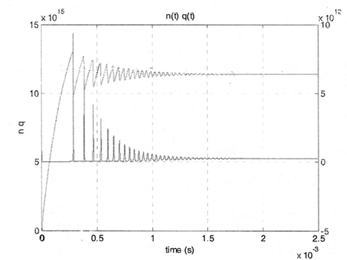
\includegraphics[width=\linewidth]{p3.png}
        % \caption{Зависимость инверсии населенности n(t) от полного числа фотонов в резонаторе q(t) в разных временных масштабах}
        \label{fig:image1}
    \end{minipage}
    \hfill
    \begin{minipage}{0.45\textwidth}
        \centering
        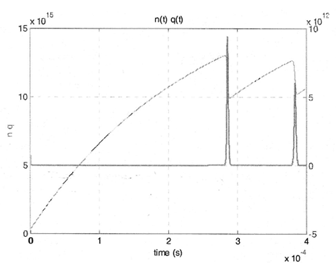
\includegraphics[width=\linewidth]{p4.png}
        % \caption{Второй рисунок}
        \label{fig:image2}
    \end{minipage}
    \caption{Зависимость инверсии населенности n(t) от полного числа фотонов в резонаторе q(t) в разных временных масштабах}
\end{figure}

\section{Экспериментальная установка}

Часть экспериментальной установки показана ниже:

\newpage

\begin{figure}[h]
    \centering
    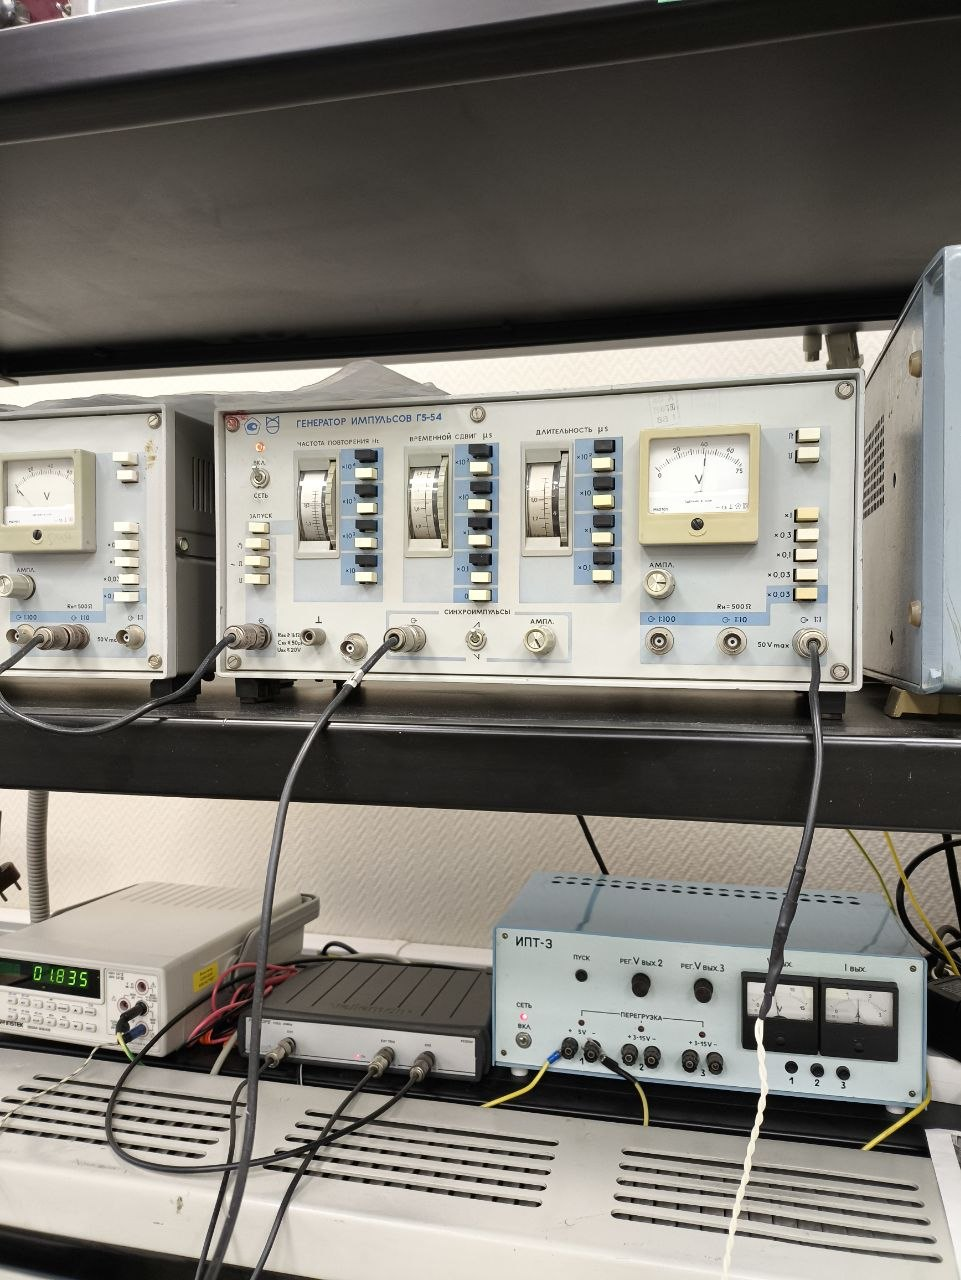
\includegraphics[width=8cm]{p1.jpg}
    \caption{Часть экспериментальной установки}
    \label{img_energy_levels}
\end{figure}


\section{Ход работы}









\end{document}
